\scanpage{104}

\uline{Théorème} \textcircled{1} Soit $N$ une norme de Schatten sur $R^{(\underline N)}$, \deleted{Soient $E$ et $F$}\inserted{pour tout couple $(E,F)$ de} deux espaces de \deleted{Banach}\inserted{Hilbert}, \deleted{posons}\inserted{et} pour $u\in L_0(E,F)$, posons

\margin{\begin{tikzpicture}[x=1cm,y=1cm]\draw[line width=.2pt] (0,0)--(.03,-.9);\end{tikzpicture}}
\[
N(u)=N((\rho_i(u)))\tag*{(18)}
\]

et pour $u\in L(E,F)$

\margin{\begin{tikzpicture}[x=1cm,y=1cm]\draw[line width=.2pt] (0,0)--(.12,-3.3);\end{tikzpicture}}
\[
N(u)=\underset{\substack{v\in F'\otimes E\\N^\circ(u)\leq 1}}{\operatorname{Sup}}|\operatorname{Tr}vu|\tag*{(19)}
\]

Cette deuxième expression coïncide avec la précédente sur $L_0(E,F)$. Soit $L^N(E,F)$ le sous-espace de $L(E,F)$ formé des $u$ tels que $N(u)<+\infty$, alors $N$ est une norme sur $L^N(E,F)$, qui en fait un espace de Banach. \deleted{L'adhérence \inserted{$L_N(E,F)$} de $E'\otimes F$ dans cet \unsure{espace est} l'espace des $u\in L_0(E,F)$ tels que} \inserted{Si $u\in L_0(E,F)$, alors on} a $u\in L^N(E,F)$ si et seulement si $(\rho_i(u))\in\ell^N$, et alors on a (18). \deleted{\unsure{N}} L'adhérence \inserted{$L_N(E,F)$} de $E'\otimes F$ dans $L^N(E,F)$ est l'ensemble des op. \deleted{\unsure{cpts}} $u\in L_0(E,F)$ tels que $(\rho_i(u))\in\ell_N$.

\margin{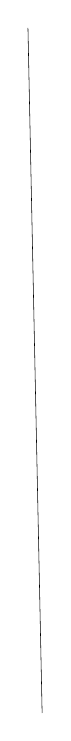
\begin{tikzpicture}[x=1cm,y=1cm]\draw[line width=.2pt] (0,0)--(.18,-8.7);\end{tikzpicture}}
\textcircled{2} On a

\[
\boxed{N(u)=N(u^*)}\boxed{\deleted{\unsure{N(u)}}}\tag*{\textcircled{20}}
\]

et par suite $u\in L^N(E,F)\mathrel{\textcolor{red}{\underline{\textcolor{black}{=}}}}u^*\in L^N(F,E)$
\margin{\deleted{\unsure{$\Longleftrightarrow u\in L^N(E,F)$|sur $L^N(E,F)$}}\quad\textcolor{red}{?}}
\inserted{de $=$} $u\in L_N^c(E,F)\mathrel{\textcolor{red}{\underline{\textcolor{black}{\Longleftrightarrow}}}}u^*\in L_N(F,E)$. On a

\[
\begin{aligned}
N(uv)&\leq\lVert u\rVert N(v)\\
N(uv)&\leq\lVert v\rVert N(u)
\end{aligned}\tag*{\textcircled{21}}
\]

si $u\in L(E,F)$, $v\in L(F,G)$. \deleted{\unsure{Donc}} En composant à gauche ou à droite un op. \deleted{$\in L^N($} du type $\ell^N$ (resp$^t$ $\ell_N$) avec un opérateur \deleted{de type} \textcolor{red}{\uline{\textcolor{black}{continu}}}, on obtient un op. du type $\ell^N$ (resp.t $\ell_N$).
\margin{\begin{tikzpicture}[x=1cm,y=1cm,line cap=round]\draw[red!70!brown,line width=.4pt] (0,.56)..controls(.015,.47)and(.045,.40)..(.035,.36)..controls(.025,.33)and(.07,.32)..(.075,.35);\draw[red!50!brown,line width=.25pt] (.075,.35)..controls(.16,.37)and(.16,.16)..(.11,.09)..controls(.07,.07)and(.11,.02)..(.10,0)..controls(.11,.04)and(.16,.10)..(.16,.13);\end{tikzpicture}}
\inserted{$N(u)$ est fonction croissante sur l'ens. des hermitiens positifs dans $L_0(E)$.}

\textcircled{3} \deleted{\textcircled{4}} Si $N,N',N''$ sont \deleted{\unsure{deux|une}}\inserted{des} normes de Schatten telles que

\[
\text{\unsure{p.|q.}}\qquad\boxed{N(xy)\leq N'(x)N'(y)}\tag*{\textcircled{22}}
\]

pour $x,y\in R^{(\underline N)}$, alors on a, pour $u\in L(E,F)$, $v\in L(F,G)$,

\[
N(vu)\leq \unsure{N'(v)|N'v)}N''(u)\tag*{\textcircled{23}}
\]

donc si $u\in L^{N'}(E,F)$, $v\in L^{N''}(E,F)$, alors $vu\in L^N(E,F)$, et si on a \inserted{de plus} $u\in L_{N'}(E,F)$ ou $v\in L_{N''}^{\unsure{\deleted{N}|*}}(E,F)$, on aura $=$ $vu\in L_N(E,F)$, -- En particulier, on aura, pour $u\in L(E,F)$, $v\in L(F,\unsure{G|E})$

\[
\lVert vu\rVert_1\leq N(u)N^\circ(v)\tag*{\textcircled{24}}
\]

donc si $u\in L^N(E,F)$, $v\in L^{N^\circ}(F,\unsure{G|E})$, on a $vu\in L^1(E,\unsure{E|G})$, et

\[
|\operatorname{Tr}vu|\leq N(u)N^\circ(v).\tag*{\textcircled{25}}
\]

\margin{105}

